%%%%%%%% ICML 2021 EXAMPLE LATEX SUBMISSION FILE %%%%%%%%%%%%%%%%%

\documentclass{article}

% Recommended, but optional, packages for figures and better typesetting:
\usepackage{microtype}
\usepackage{graphicx}
\usepackage{subfigure}
\usepackage{booktabs} % for professional tables

% hyperref makes hyperlinks in the resulting PDF.
% If your build breaks (sometimes temporarily if a hyperlink spans a page)
% please comment out the following usepackage line and replace
% \usepackage{icml2021} with \usepackage[nohyperref]{icml2021} above.
\usepackage{hyperref}

% Attempt to make hyperref and algorithmic work together better:
\newcommand{\theHalgorithm}{\arabic{algorithm}}

% Use the following line for the initial blind version submitted for review:
% \usepackage{icml2021}

% If accepted, instead use the following line for the camera-ready submission:
\usepackage[accepted]{icml2021}

% The \icmltitle you define below is probably too long as a header.
% Therefore, a short form for the running title is supplied here:
\icmltitlerunning{Hierarchical, multi-label prediction for automated cell type identification}

\begin{document}

\twocolumn[
\icmltitle{Hierarchical, multi-label prediction for automated cell type identification}

% It is OKAY to include author information, even for blind
% submissions: the style file will automatically remove it for you
% unless you've provided the [accepted] option to the icml2021
% package.

% List of affiliations: The first argument should be a (short)
% identifier you will use later to specify author affiliations
% Academic affiliations should list Department, University, City, Region, Country
% Industry affiliations should list Company, City, Region, Country

% You can specify symbols, otherwise they are numbered in order.
% Ideally, you should not use this facility. Affiliations will be numbered
% in order of appearance and this is the preferred way.
% \icmlsetsymbol{equal}{*}

\begin{icmlauthorlist}
\icmlauthor{Iwijn Voeten}{ugent}
\icmlauthor{Klaas Goethals}{ugent}
\end{icmlauthorlist}

\icmlaffiliation{ugent}{Department of Applied mathematics, computer science and statistics, Ghent University, East-Flanders, Belgium}

\icmlcorrespondingauthor{Voeten Iwijn}{iwijn.voeten@ugent.be}
\icmlcorrespondingauthor{Goethals Klaas}{klaas.goethals@ugent.be}

% You may provide any keywords that you
% find helpful for describing your paper; these are used to populate
% the "keywords" metadata in the PDF but will not be shown in the document
\icmlkeywords{Machine Learning, Hierarchical, classification}

\vskip 0.3in
]

% this must go after the closing bracket ] following \twocolumn[ ...

% This command actually creates the footnote in the first column
% listing the affiliations and the copyright notice.
% The command takes one argument, which is text to display at the start of the footnote.
% The \icmlEqualContribution command is standard text for equal contribution.
% Remove it (just {}) if you do not need this facility.

\printAffiliationsAndNotice{}  % leave blank if no need to mention equal contribution
% \printAffiliationsAndNotice{\icmlEqualContribution} % otherwise use the standard text.

\begin{abstract}
This study researches the use of different high level methods to classify cells based on gene expression data.
Cell types are hierarchical in nature, thus it would seem logical to use the hierarchical structure as extra data in our machine learning models. 

In this paper we build different kinds of hierarchical models and compare them to regular flat classifiers where the natural hierarchy is not taken into account during training. Our findings are that hierarchical models can be trained faster than flat models while getting the same accuracy. 

However, when training hierarchical models, the hierarchy must be limited to prevent the loss of accuracy. A deep hierarchical model performs worse than a regular flat classifier.
%A \textit{flat} classifier can be used, as well as different hierarchical-style methods.
%Results show that hierarchical classifiers are often faster, but accuracy can decrease rapidly.
\end{abstract}

\section{Problem description}

%In biology, cell types are used to label cells.
Cells are divided into types depending on morphological and phenotypical features.
It's obvious that these types can be divided in groups, and therefore hierarchically structured.
A simple example of such a hierarchical structure can be seen in Figure \ref{cell-hyr}.

\begin{figure}[ht]
\vskip 0.2in
\begin{center}
\centerline{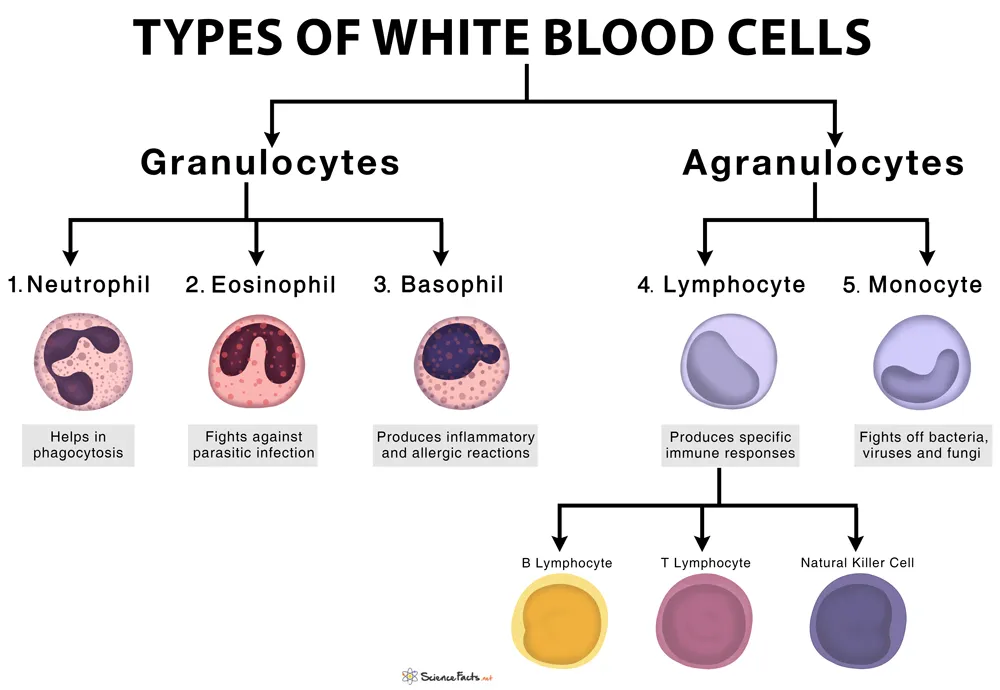
\includegraphics[width=\columnwidth]{images/cell-hyr.png}}
\caption{Cell type tree of the classification made in white blood cells \cite{cell-hyr}}
\label{cell-hyr}
\end{center}
\vskip -0.2in
\end{figure}

The problem at hand is to classify a cell based on its gene expression data.
This research focuses on different hierarchical models and what their advantages and disadvantages might be. 

\section{Related work}

A few different methods to classify hierarchical data already exist.

The most simple solution is a so-called flat, non-hierarchical classifier. This can be any multi-label machine learning classifier. It is used to classify the distinct cell types, essentially the leafs of the tree, as labels.

On the other hand, there are multiple local hierarchical models.
Such a hierarchical model is a model consisting of multiple \textit{base} models structured in a hierarchy.
These hierarchic models can be divided into three main categories, as Weiss (2020) describes:
\textbf{Local classifier per node}, \textbf{Local Classifier per Parent Node (LCPN)} and \textbf{Local Classifier per Level (LCL)}.

\subsection{Local Classifier per Node (LCN)}
\label{LCN}
\begin{figure}[ht]
\vskip 0.2in
\begin{center}
\centerline{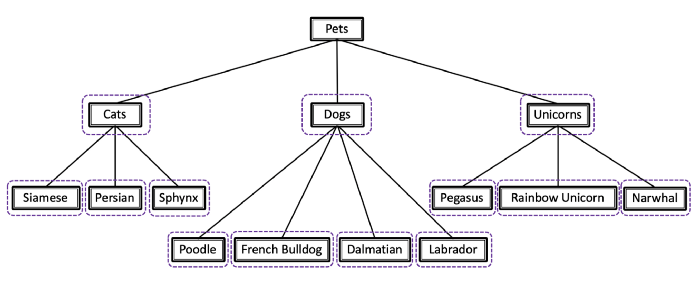
\includegraphics[width=\columnwidth]{images/lcn.png}}
\caption{Visual representation of how a Local Classifier per Node model works. The circled nodes each have a classifier.}
\label{lcn}
\end{center}
\vskip -0.2in
\end{figure}

In this classifier, every node in the tree (except for the root) has a binary classifier.
Each classifier will decide whether that specific label belongs to the given data or not.

In Figure \ref{cell-hyr} there would be 10 binary classifiers: one for every tree node except the root.
A single data sample could then be classified by those classifiers as followed: the \textit{Granulocytes}-classifier and the \textit{Eosinophil}-classifier return a positive ('true'), all other classifiers return a negative.
It can then be concluded that that sample belongs to the \textit{Eosinophil} cell type. 

\subsection{Local Classifier per Parent Node (LCPN)}
\label{LCPN}
In this classifier, every \textbf{parent node} in the tree has a multi-label classifier.
Each classifier will decide which of the node's children belongs to the given data.

In Figure \ref{cell-hyr} there would be 4 classifiers: one for every node that is not a leaf.
A single data sample could then be classified by those classifiers as followed: the  root classifier decides the best label is \textit{Agranulocytes} and the \textit{Agranulocytes}-classifier returns \textit{Monocyle}.
In this case, we \textit{could} disregard the other classifiers and decide on \textit{Monocyle}, but that is not necessary.

\subsection{Local Classifier per Level (LCL)}
\label{LCL}
This classifier has a multi-label classifier for each level in the tree. The classifier for level L can classify in each class of level L, no matter what the output is of the previous level classifier. This can however give nonsensical results. 

For example, let's look at Figure \ref{cell-hyr} again. The L1 classifier could give \textit{Granulocytes} as their output. In the next step, the L2 classifier could give \textit{Monocyte}, a child of  \textit{Agranulocytes}, as it's output. These 2 predictions together make no sense. \\

In addition to these local methods, global ones exists, like Hierarchical Multi-Label Classification Networks (HMCN). This technique involves solving the problem with a neural network \cite{hmcn}. Another method is using a genetic algorithm \cite{genetic}. We will leave these to the side and compare the local methods.

\section{Material and methods}

%Here you describe all the algorithms you experimented with, possibly also novel techniques you designed yourself.
Multiple hierarchical methods were experimented with and tested.
An attempt to parallelise a hierarchical model was also made.

\subsection{Data and filtering}

We had two datasets at our disposal.
One is an Allen Mouse Brain (AMB) dataset.
The other one is based on a BAL (Bronchoalveolar Lavage) sample of a COVID patient.

These datasets are \textit{count tables}.
They consist of \textit{rows} that each represent a cell.
For each cell, there are counts that describe which genes are expressed in the cell.
So essentially the data is a table with a row representing a cell and a column representing a gene expression.

Some filtering processes were applied to this data.
Columns consisting of all zeros were removed because they have no impact on the machine learning model.
For example, for the "covid-BAL" dataset, approximately 14\% of all columns were all zeros.
In addition, rows with few non-zero numbers were removed.

\begin{figure}[ht]
\vskip 0.2in
\begin{center}
\centerline{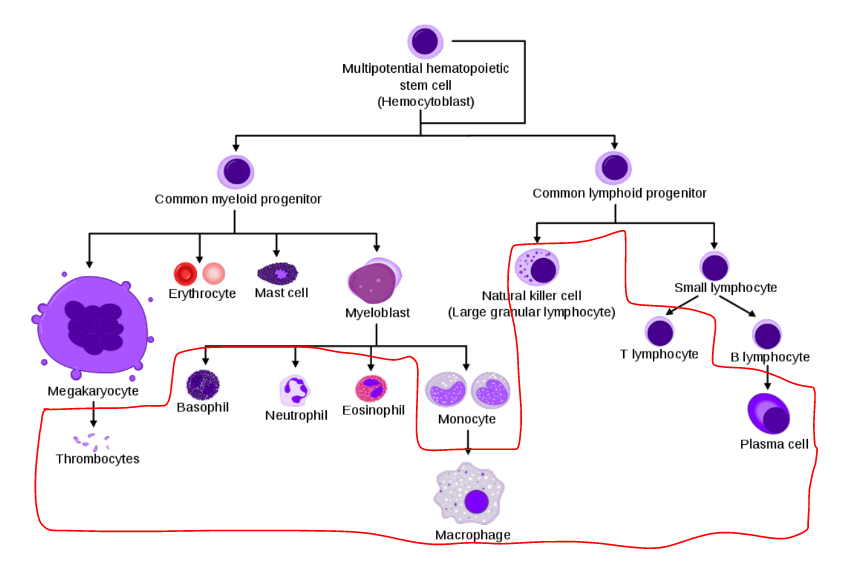
\includegraphics[width=\columnwidth]{images/flat.png}}
\caption{Visual representation of how a flat classifier works. The leaf nodes are the classes, the hierarchy makes no difference.}
\label{icml-historical}
\end{center}
\vskip -0.2in
\end{figure}

\subsection{Flat classifier}

A flat classifier was the baseline we compared all hierarchical models against. This is because there is no point in creating a more complex hierarchical model if the same can be done with a much simpler non-hierarchical model.

A \textbf{Linear Support Vector Classifier (SVC)}, provided by \verb|scikit-learn| is used to classify the data \cite{scikit-learn}.
The same kernel is also used in all below methods for consistency and because comparing different kernels is not the focal point of this research.

\subsection{Local Classifier per Parent Node (LCPN)}
Local Classifier per Parent Node is explained in section \ref{LCPN}. A full hierarchical implementation was implemented as well as a partial hierarchical model where the depth of the tree was intentionally limited.

\subsubsection{Full depth}
\begin{figure*}[ht]
\vskip 0.2in
\begin{center}
\centerline{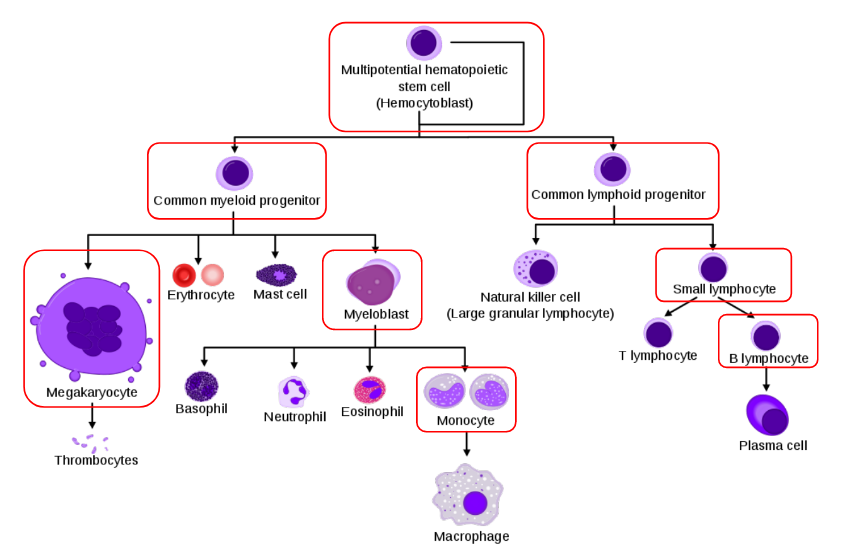
\includegraphics[width=5in]{images/full-hyr.png}}
\caption{Visual representation of how a full depth hierarchical classifier works. Each circles node has a classifier.}
\label{full-hyr}
\end{center}
\vskip -0.2in
\end{figure*}

The full depth tree works as seen in Figure \ref{full-hyr}. Each node which is not a leaf node in the tree has a multi-label classifier that can further classify the results. The con of this approach is the fact that, for example, the \textit{Small lymphocyte} node might have a classifier that was trained on very little data. 

If only 1 percent of your dataset are cells that belong to the \textit{Small lymphocyte} class, you can only use 1 percent of your data to train the classifier in the \textit{Small lymphocyte} node.

\subsubsection{Limited depth}
\begin{figure}[ht]
\vskip 0.2in
\begin{center}
\centerline{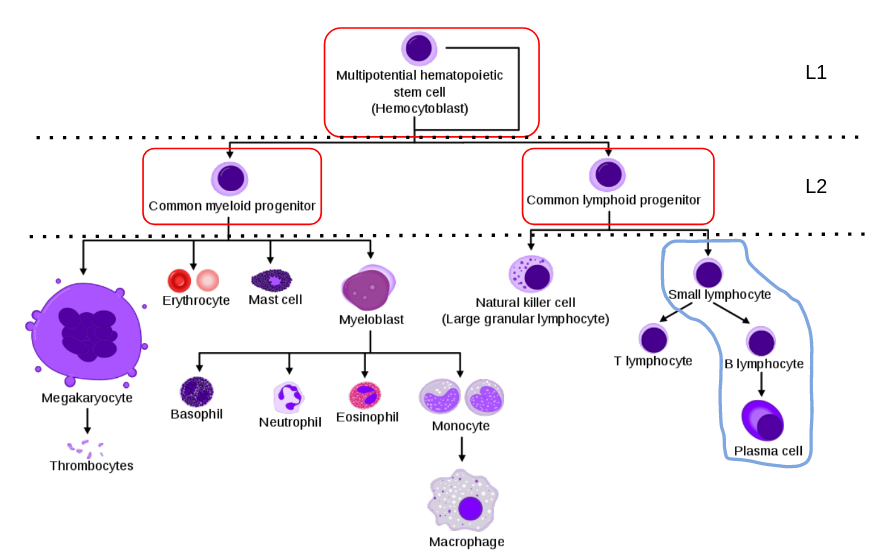
\includegraphics[width=\columnwidth]{images/partial-hyr.png}}
\caption{Visual representation of how a limited depth hierarchical classifier works. The circled nodes have a classifier. The path circled blue shows how that path is seen as 1 result that the L2 classifier can return.}
\label{limited-hyr}
\end{center}
\vskip -0.2in
\end{figure}

The limited depth tree works as seen in Figure \ref{limited-hyr}. In this model, we don't train a classifier for each non-leaf node, but only for the non-leaf that are high enough in the tree. This way, we have a bigger chance of training the classifier on a large chunk of data. 

We performed tests on the Allen Mouse Brain dataset with a limited depth of 3, meaning a prediction would go through exactly 3 different multi-label classifiers to end up at its final prediction.

For example, the classifier in the \textit{Common lymphoid progenitor} now classifies an entry into either \textit{Natural killer cell}, \textit{T lymphocyte} or \textit{Plasma cell}. While in the full depth tree, it would classify into \textit{Natural killer cell} and \textit{Small lymphocyte}. When  \textit{Small lymphocyte} would be predicted, it would further classify with an under trained classifier.

\subsection{Local Classifier per Level modified}
\begin{figure}[ht]
\vskip 0.2in
\begin{center}
\centerline{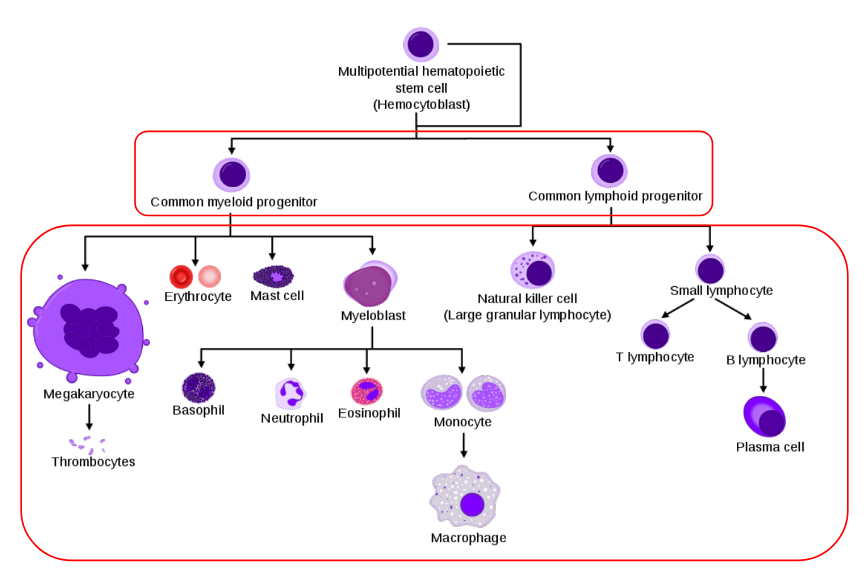
\includegraphics[width=\columnwidth]{images/lcl.png}}
\caption{Visual representation of how a Local Classifier per Level model. Each level has a classifier. The bottom level is 1 big classifier that results in one of the leaf nodes because the depth of the tree varies.}
\label{LCL}
\end{center}
\vskip -0.2in
\end{figure}

\begin{figure*}[ht]
\vskip 0.2in
\begin{center}
\centerline{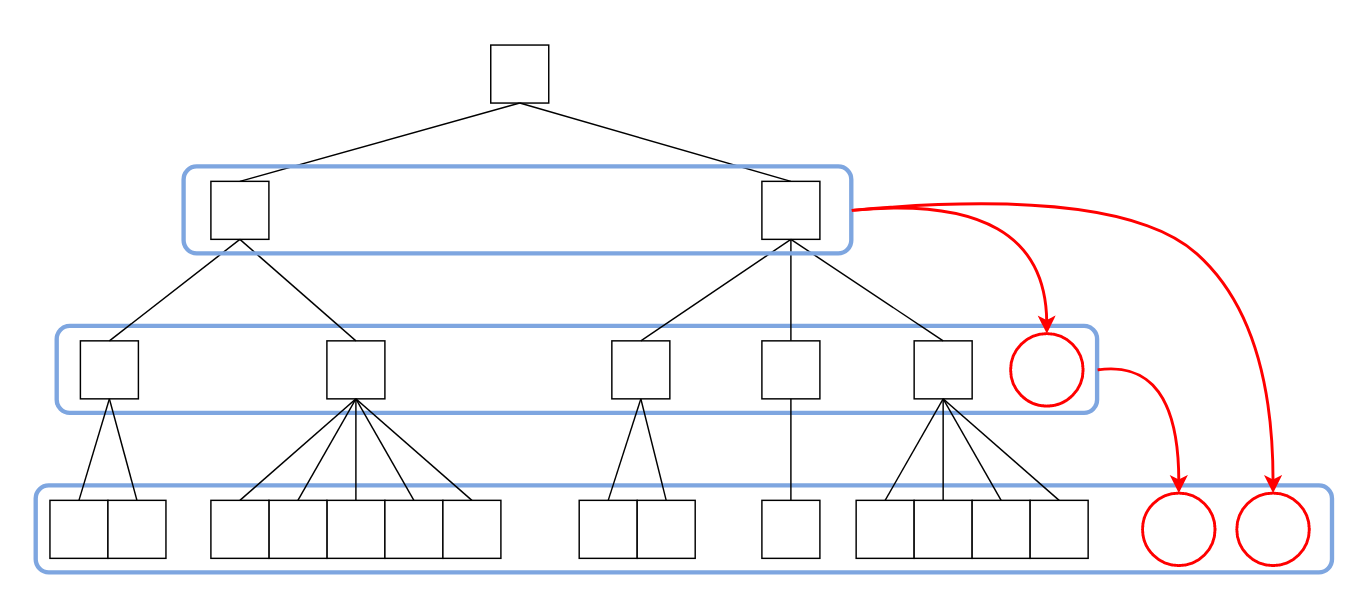
\includegraphics[width=5in]{images/lcl-modified.png}}
\caption{Visual representation of how a Local Classifier per Level modified model works. Each layer has a classifier represented as the blue circled areas. The output of each layers' classifier, represented as red circles, is given as input for the classifiers of all following layers.}
\label{LCL-modified}
\end{center}
\vskip -0.2in
\end{figure*}

The problems this modified classifier was attempting to solve were:
\begin{itemize}
    \item LCL can generate nonsensical predictions
    \item LCPN can miss classify early on in the tree, and this is never corrected
\end{itemize}

The idea is that we sometimes want to have a nonsensical classification. When a previous classification was wrong, we want it to make a "nonsensical" classification, which chooses a different path in the tree than the wrong prediction. 

For example, let's say we are trying to classify a \textit{Plasma cell}. When using a hierarchical model as shown in Figure \ref{full-hyr} a miss classification into the \textit{Common myeloid progenitor} node would mean a definite miss classification. But when using a model like show in Figure \ref{LCL}, an initial miss classification into the \textit{Common myeloid progenitor} node wouldn't make a difference for the final classification.

It might be a good idea to try and combine these two properties and create a hybrid where a previous classification can be useful information for the next classification.

This was attempted by making a classifier as shown in Figure \ref{LCL-modified}. Each layer feeds its result to all following layers. This makes it so that a layer can decide for itself if it thinks one or more previous layer(s) might have miss classified.

\subsubsection{Training LCL modified}
Training this model had its challenges. This is because for Layer x to be trained, you need to know the output of all previous already trained layers.

To explain how a training cycle goes in this model, we will assume we are training the model in Figure \ref{LCL-modified} and thus 3 layers need to be trained.
First, we divide the training set up in 3 parts. 
Each part will be used to train a layer.
We use the first part to train the first layer as we would any multi-label classifier.

We then use this trained classifier to predict the outcomes for the second part of the dataset. These predictions, together with the gene expression data, are then used to train the second layer. As you can see in Figure \ref{LCL-modified}, the second layer needs the prediction of the first layer.

Then finally we use the 3rd part of the training dataset, we feed this data to the first layer, then we feed it to the second layer together with what the first layer predicted. 
Now this third part has 2 extra columns, namely the prediction of the first layer, and the prediction of the second layer, this can now be used to train the third layer classifier.

This strategy should in theory now be trained to also detect when an early on classification goes wrong. The layer 2 classifier might be able to learn the right strategy when it predicts something contradictory to the layer 1 classifier.

On a tree where leaf nodes are not all at the same depth, a limited hierarchical strategy is used, similar to what is explained in section \ref{limited-hyr}.


\subsection{Parallelisation of hierarchical models}

The hierarchical models using local methods consist of multiple models.
For the LCPN technique, they should be able to be implemented with parallelisation.
The local classifiers on the same level do not depend on each other.
They can therefore be trained completely separate and possibly at the same time on different threads or processes.

For the LCL approaches, the same property holds: in theory the training process can be parallelised.
It is however not possible for the modified LCL method we proposed.
Using that strategy, every classifier depends on the ones higher in the hierarchy.

This works in theory, but in this research project we were not able to successfully implement this.
The attempt to implement this with python and the \verb|multiprocess| python library \cite{multiprocessing1} \cite{multiprocessing2} failed.
The use of \verb|Pool| to spawn multiple worker processes performs badly because the specified data is copied on each spawn.
For big datasets, this makes parallelisation infeasible.
To make parallelisation work, the memory should be shared in some way.

\section{Results}

The above methods were tested on the Allen Mouse Brain dataset using 2-fold validation.
As can be seen in Table \ref{results}, no hierarchical model performed significantly better than the flat model. In fact, a deep hierarchical model performed worse than the flat classifier.

The Local Classifier per Level modified discussed in section \ref{LCL-modified} is a little bit slower than the flat classifier and unfortunately did not perform better.

A partial hierarchical model is the best option. It offers faster training, and no loss of accuracy and F1 score.
On average, this method offered a $18.8\%$ time decrease.

In conclusion, hierarchical models can be used to speed up training, but don't offer any advantage in making a more accurate prediction.

\begin{table}[t]
\caption{Accuracy and F1 scores weighted-average and macro-average for different models tested on the Allen Mouse Brain dataset using 2-fold validation. The limited hierarchical model had a depth of 3.}
\label{results}
\vskip 0.15in
\begin{center}
\begin{small}
\begin{sc}
\begin{tabular}{@{}p{27mm}p{14mm}p{14mm}p{14mm}@{}}
\toprule
                                & Accuracy & F1 macro-averaged & F1 weighted-averaged \\ \midrule
Flat classifier\newline                 & 0.9017   & 0.8421            & 0.8997              \\

Limited \newline hierarchical \newline classifier (LCPN)\newline  & 0.9020   & 0.8443            & 0.9001              \\

Full \newline hierarchical \newline classifier (LCPN)\newline     & 0.4720   & 0.6030            & 0.4797               \\
LCL modified \newline classifier & 0.8673 & 0.7703 & 0.8618 \\ \bottomrule
\end{tabular}
\end{sc}
\end{small}
\end{center}
\vskip -0.1in
\end{table}

\section{Discussion and future work}

Implementing the Local Classifier per Node (LCN) as explained in section \ref{LCN} is a definite further research opportunity. 

Another research opportunity is applying the limited hierarchical classifier with different depths and on many datasets. This way, a mathematical relationship might be found between the size of the data and the optimal depth of this model.

\section*{Acknowledgements}

We would like to thank Lauren Theunissen for providing the two datasets.
We were very grateful that the data was ready to use.

In addition, we would like to thank Daniel Peralta, Arne Gevaert, David Novak and Joris Roels for the efforts put into the practical sessions.

And finally we would like to thank Yvan Saeys for the support, feedback and theoretical lectures.


% In the unusual situation where you want a paper to appear in the
% references without citing it in the main text, use \nocite
%\nocite{langley00}
\nocite{hyr-types-blog}
\nocite{source1}
\nocite{source2}
\nocite{source3}
\nocite{source4}

% break url in references
% https://tex.stackexchange.com/a/344711
\def\UrlBreaks{\do\/\do-}

\bibliography{main}
\bibliographystyle{icml2021}

\end{document}


% This document was modified from the file originally made available by
% Pat Langley and Andrea Danyluk for ICML-2K. This version was created
% by Iain Murray in 2018, and modified by Alexandre Bouchard in
% 2019 and 2021. Previous contributors include Dan Roy, Lise Getoor and Tobias
% Scheffer, which was slightly modified from the 2010 version by
% Thorsten Joachims & Johannes Fuernkranz, slightly modified from the
% 2009 version by Kiri Wagstaff and Sam Roweis's 2008 version, which is
% slightly modified from Prasad Tadepalli's 2007 version which is a
% lightly changed version of the previous year's version by Andrew
% Moore, which was in turn edited from those of Kristian Kersting and
% Codrina Lauth. Alex Smola contributed to the algorithmic style files.
